\documentclass[10pt,journal]{IEEEtran}
\usepackage{amsmath,amssymb}
\usepackage{amsthm}
\usepackage{booktabs}
\usepackage{algorithm}
\usepackage{algpseudocode}
\usepackage{graphicx}
\usepackage{float}
\usepackage{url}
\usepackage{xcolor}
\usepackage{cite}
\newtheorem{definition}{Definition}
\newtheorem{lemma}{Lemma}
\newtheorem{proposition}{Proposition}
\newtheorem{theorem}{Theorem}
\newtheorem{corollary}{Corollary}
\theoremstyle{remark}
\newtheorem{remark}{Remark}
\newcommand{\sys}{\mbox{QuantGhost}}

\begin{document}
\title{\sys: Deployment-Robust Weight Steganography and a Capacity--Robustness--Stealth Trilemma}
\author{Eko~Arip~Winanto,~Mohd~Yazid~Idris,~Kurniabudi,~and~Febby~Tri~Ramadhanti%
\thanks{E. A. Winanto is with the Faculty of Computing, Universiti Teknologi Malaysia, Johor Bahru 81310, Malaysia, and the Department of Computer Engineering, Universitas Dinamika Bangsa, Jambi 36138, Indonesia (e-mail: winanto@graduate.utm.my; ORCID: \mbox{0000-0003-3274-1885}).}%
\thanks{M. Y. Idris is with the Faculty of Computing and MaGIC-X, Universiti Teknologi Malaysia, Johor Bahru 81310, Malaysia (ORCID: \mbox{0000-0001-7702-6610}).}%
\thanks{Kurniabudi is the corresponding author, with the Master of Information System program, Universitas Dinamika Bangsa, Jambi 36138, Indonesia (e-mail: kurniabudi@unama.ac.id; ORCID: \mbox{0000-0001-9073-8858}).}%
\thanks{F. T. Ramadhanti is with the Distance Learning Master's Program in Technology and Vocational Education, Universitas Negeri Yogyakarta, Yogyakarta 55281, Indonesia.}%
\thanks{This work was funded by Universitas Dinamika Bangsa and supported by MaGIC-X, Universiti Teknologi Malaysia.}}
\maketitle
\bstctlcite{IEEEexample:BSTcontrol}

\begin{abstract}
Pre-trained networks circulate as shared artifacts, so a tampered checkpoint on a popular
hub reaches every downstream user. Prior weight-steganography attacks hide megabytes in
float32 mantissas, yet their reported capacity rests on an untested assumption: that the
model is deployed exactly as published. It rarely is. Before reaching an edge or medical
(IoMT) device a model is quantized to INT8, pruned and fine-tuned, and we confirm on real
networks that these steps erase mantissa-bit payloads, while a faithful MaleficNet
survives them only at watermark-scale capacity. We present \sys, a quantization-aware
embedding that writes each payload bit into the INT8 code quantization produces, so it
survives by construction, and places each weight at a random point in its code bin to keep
the mantissa distribution benign; redundant coding carries the payload through pruning and
fine-tuning. \sys{} revises the picture: a $3.2$\,MB payload survives INT8 on ResNet-50
($99.9999\%$) and the production PyTorch kernel byte-exactly, at a cost of $0.19$ accuracy
points on ResNet-56, and evades the Model X-Ray detector on a diverse population
($0.50$ vs.\ $0.81$ for prior art). A capacity-robustness-stealth trilemma we prove bounds
any stealthy, quantization-robust, permutation-invariant channel to
$\sum_\ell k_h k_w$ bits, so a faithful neuron permutation erases the high-capacity payload
but a $196$-bit invariant channel survives to carry an out-of-band key; a proposed
sub-quantum residual detector flags the basic attack (AUC $0.98$--$1.0$) but an adaptive
attacker reaches chance. Deployment sanitization alone is therefore incomplete, and the
trilemma gives defenders a concrete target.
\end{abstract}

\begin{IEEEkeywords}
Neural network steganography, stegomalware, model supply chain, quantization, steganalysis, deep learning security, QuantGhost.
\end{IEEEkeywords}

% =====================================================================
\section{Introduction}\label{sec:intro}
Sharing pre-trained models is now the default way to build machine-learning systems.
Practitioners pull a checkpoint from a hub, adapt it, and ship it. That convenience
turns the model file itself into a supply-chain asset, and a tampered file propagates
to everyone who reuses it, the same dynamic that makes poisoned packages and
trojaned binaries dangerous, transplanted into the weight space of a network
\cite{gu2017badnets,liu2018trojaning,digregorio2026insecurity}. The carrier is generous: a float32
weight devotes most of its mantissa to precision the task never needs, and StegoNet
\cite{liu2020stegonet}, EvilModel \cite{wang2021evilmodel,wang2022evilmodel2} and
MaleficNet \cite{hitaj2022maleficnet,hitaj2025trust} exploit exactly that slack to
hide megabytes of payload with accuracy loss below one percent.

These attacks assume a static artefact, a condition the deployment pipeline violates. A
model is almost never deployed bit-for-bit as published. On the way to a phone, a sensor, or a bedside IoMT
monitor it is compressed: post-training INT8 quantization \cite{jacob2018quantization},
magnitude or structured pruning \cite{han2015learning,han2016deepcompression}, and a
round of fine-tuning on local data. We show in Section~\ref{sec:motiv}, on real
networks, not toy ones, that this pipeline annihilates a mantissa-bit payload:
recovery falls to a coin flip at every embedding depth. Worse for the attacker, the
very same transforms have been put forward as defenses, alongside neuron permutation
(NeuPerm), which shuffles channel order using the network's permutation symmetry and
scrambles any position-dependent payload at no accuracy cost
\cite{gilkarov2025neuperm}. Detection has matured in parallel: Model X-Ray casts the
weights to a grayscale image and learns, from a handful of examples, to tell stego
from benign \cite{gilkarov2026modelxray}.

So the question that has not been answered is sharp. \emph{Can a payload survive the
full deployment pipeline and still be stealthy and accuracy-preserving?} We answer it
constructively, but the more durable contribution is what the answer exposes: a
fundamental three-way limit, a \emph{capacity-robustness-stealth trilemma}, that
constrains every weight-embedding scheme, ours and prior watermarking alike. We develop
the work in three movements.

First, the attack, which we name \sys. Rather than hiding in the mantissa, it writes
each payload bit into the INT8 code that quantization will produce, so re-quantization
recovers it exactly (Section~\ref{sec:method}). Stealth follows from two design choices:
the payload is encrypted, and each weight is placed at a random point \emph{inside} the
bin that encodes its bit. The mantissa keeps its natural law, and a byte-image detector has nothing to
latch onto. Redundancy across many weights, decoded by majority vote, carries the
payload through pruning and fine-tuning.

Second, and at the centre of the paper, a limit. We formalize and prove the
capacity-robustness-stealth trilemma (Section~\ref{sec:trilemma}): no embedding can be
simultaneously high-capacity, permutation-invariant, and stealthy-quantization-robust.
The argument is short once the right object is in view. Once an embedding is stealthy
and quantization-robust, the only identity a weight keeps under neuron permutation is
its coarse code, and codes that share a permutation orbit cannot index a high-capacity
positional message. The permutation-invariant channel is therefore bounded by
$\sum_\ell k_h^{(\ell)} k_w^{(\ell)}$ bits, a quantity four to five orders of magnitude
smaller than the positional channel. Our construction attains this bound to the bit, and
because the limit is a property of the permutation group rather than of our encoder, the
same ceiling constrains any stealthy, quantization-robust permutation-invariant scheme; we
prove it for the weight-embedding channel and conjecture the analogue for robust watermarking
under the same group (Section~\ref{sec:trilemma}).

Third, the consequence for defense. A faithful neuron permutation, verified
function-preserving to machine precision on a real ResNet-18, does destroy the
high-capacity payload. But the small invariant channel survives untouched, and we
demonstrate the consequence end to end: after the full INT8, pruning, and NeuPerm
pipeline, a $128$-bit AES key recovered from the invariant channel decrypts a ciphertext
delivered out of band and returns the payload byte-exactly, even though the high-capacity
payload embedded in the weights is itself gone. What survives NeuPerm is thus a bootstrap
key channel, not an in-weight payload. Sanitization that stops at NeuPerm is therefore
incomplete, and we describe what closing the gap would take (Section~\ref{sec:defenses}).

This paper makes the following contributions:
\begin{itemize}
\item \textbf{A capacity-robustness-stealth trilemma.} For the function-preserving
  channel-permutation group of convolutional and dense layers, we formalize and prove that
  no weight-embedding scheme can be high-capacity, permutation-invariant, and
  stealthy-quantization-robust at once: any stealthy, quantization-robust,
  permutation-invariant channel carries at most $\sum_\ell k_h^{(\ell)} k_w^{(\ell)}$ bits.
  Our construction attains this value, so it is tight within that class; we confirm it to the
  bit on a real ResNet-18 and conjecture the analogue for robust watermarking under the same
  group.
\item \textbf{\sys, a construction that reaches the bound.} We build a
  deployment-robust, distribution-preserving embedding that occupies the
  high-capacity, stealthy, quantization-robust corner of the trilemma. It survives INT8
  quantization, pruning and fine-tuning, and we demonstrate it at $3.2$\,MB on a real
  ResNet-50 at a cost of $0.19$ percentage points of accuracy on a real ResNet-56.
\item \textbf{Why prior payloads die.} We quantify, on real models, why routine
  deployment transforms erase the payloads of prior weight-steganography attacks, and
  explain the mechanism through the quantization step size.
\item \textbf{The limit of permutation defenses, demonstrated end to end.} We implement
  a faithful, full-model neuron permutation on a real ResNet-18 and show that, although it
  erases the high-capacity in-weight payload, a $128$-bit key embedded in the invariant
  channel survives the entire INT8, pruning, and permutation pipeline; the key then decrypts
  an out-of-band ciphertext byte-exactly. We are explicit that what survives permutation is
  this bootstrap key channel rather than the in-weight payload, which is already enough to
  make permutation-based sanitization incomplete.
\item \textbf{A targeted detector and its limit.} We propose and evaluate a sub-quantum
  residual steganalyzer that detects the basic \sys{} at ROC-AUC $0.98$--$1.0$ across a
  narrow and a diverse $3000$-model zoo where byte-level steganalysis is at chance; we then
  show honestly that an adaptive attacker reaches chance on the diverse zoo, so detection
  must compose with neuron permutation to bound the channel.
\item \textbf{Generality.} We show that the attack is architecture- and domain-agnostic,
  carrying a $10.81$\,MB payload through a real Vision Transformer and surviving INT8 with
  unchanged accuracy, and that it transfers across domains through a cross-dataset study on
  network-intrusion-detection models; we then set out the requirements for a complete defense.
\end{itemize}

The remainder of the paper is organized as follows. Section~\ref{sec:related} reviews
weight steganography, steganalysis, sanitization defenses, and watermarking.
Section~\ref{sec:threat} states the threat model and Section~\ref{sec:motiv} shows why
naive payloads die in deployment. Section~\ref{sec:method} develops the proposed attack
and Section~\ref{sec:trilemma} proves the trilemma. Section~\ref{sec:setup} describes
the experimental setup and Section~\ref{sec:eval} reports the evaluation, including the
cross-dataset ablation. Section~\ref{sec:defenses} discusses defenses,
Section~\ref{sec:disc} the limitations, and Section~\ref{sec:ethics} the ethical
considerations, before Section~\ref{sec:concl} concludes.

% =====================================================================
\section{Background and Related Work}\label{sec:related}
\paragraph{Hiding payloads in weights.} StegoNet \cite{liu2020stegonet} introduced
several channels, LSB substitution, value mapping, sign and resilience coding,
and reported megabyte capacity. EvilModel \cite{wang2021evilmodel} and its successor
\cite{wang2022evilmodel2} simplified this to direct byte substitution in the
low-order mantissa and pushed capacity past $36$\,MB on AlexNet. MaleficNet
\cite{hitaj2022maleficnet} departed from raw LSB editing, spreading the payload with
CDMA-style channel coding so that it tolerates small weight changes, and its journal
extension surveys the broader ecosystem risk \cite{hitaj2025trust}. A complementary
line measures how much a given architecture can absorb before accuracy degrades
\cite{agrawal2023stegcapacity,zhang2023stegcapacity}, and a recent survey organizes
the field \cite{chaganti2021stegomalware}. What unites these works is the verbatim
assumption: none reports survival through INT8 quantization. We show
(Section~\ref{sec:motiv}) that the mantissa-LSB ones do not survive it, and, by running a
faithful MaleficNet on the same pipeline (Section~\ref{sec:maleficnet}), that its
spread-spectrum payload \emph{does} survive INT8, pruning and fine-tuning but only at
watermark-scale capacity---decaying to chance as the payload approaches one bit per weight.
The high-capacity, quantization-robust corner is the one \sys{} occupies.

\paragraph{Detecting it.} Model X-Ray \cite{gilkarov2026modelxray}
maps weights to a Grayscale-Fourpart image and trains a metric-learning
few-shot classifier \cite{snell2017prototypical,vinyals2016matching} that flags
embedded payloads from as few as six examples and down to a $25\%$ embedding rate.
Siamese and meta-learning detectors have likewise proven effective for obfuscated
malware \cite{zhu2023taskaware}. Byte-entropy thresholds and raw-byte 1D-CNNs of the
MalConv family round out the standard baseline set, and we evaluate against all of
them.

\paragraph{Sanitizing it.} Quantization and pruning are cited as incidental
countermeasures because they perturb weights, much as fine-pruning was proposed to
remove backdoors \cite{liu2018finepruning}, and content-disarming approaches neutralize
embedded payloads by rewriting the model file \cite{dubin2023disarming}. NeuPerm
\cite{gilkarov2025neuperm} makes the idea deliberate, using permutation symmetry to relabel
channels and break any position-coded payload, reportedly even in large language models, and
concurrent work likewise defends against stegomalware with permutation symmetry
\cite{torpmannhagen2025permutation}. Our trilemma speaks directly to this line: it explains
both why permutation defenses work against high-capacity positional payloads and why a
low-capacity residual channel must always survive them, which is the gap such defenses do not
yet close.

\paragraph{Robust watermarking and quantization-index modulation.} The closest relative
of \sys{} is robust DNN watermarking, and its embedding primitive is an instance of
quantization-index modulation (QIM) \cite{chen2001qim}: a payload bit selects which of two
interleaved quantizers a host sample is snapped to. Spread-transform dither modulation
\cite{li2021stdm} is a QIM scheme; fixed distribution-optimized weights
\cite{tondi2022robust} and spread-spectrum TATTOOED \cite{pagnotta2022tattooed} pursue the
same robustness by other coding. We state plainly what is, and is not, new relative to QIM.
The bit-into-code-LSB primitive of \sys{} \emph{is} QIM, and our random in-bin offset is a
form of distortion-compensated QIM (DC-QIM) \cite{chen2001qim}: DC-QIM adds a scaled
quantization-error term back to the host to lower embedding distortion, and our offset plays
the analogous role of keeping the reconstructed weight off the lattice points. The one
deliberate difference is that we draw the offset \emph{uniformly} within the bin rather than
deriving it from the host value as classical DC-QIM would; a host-derived offset would
preserve the per-weight value most faithfully, but a uniform offset is what makes the
\emph{aggregate} mantissa law match a benign population (Section~\ref{sec:method}), which is
the property a learned steganalyzer reads. What \sys{} contributes beyond QIM is therefore
not the embedding primitive but (i) the deployment setting, post-hoc insertion recovered by
an adversary after an \emph{unknown} transform chain rather than an owner-read watermark fixed
at training time, and (ii) the capacity analysis under the function-preserving neuron-permutation
group, which the signal-processing QIM literature does not consider. On usage rather than
capability, published QIM watermarks typically carry a few kilobits for ownership whereas we
operate QIM at one bit per weight for payload delivery; this is an operating-point choice, not
a capacity limit of QIM. The trilemma of Section~\ref{sec:trilemma} bounds the
permutation-invariant regime, and we conjecture an analogous bound for QIM watermarking under
the same group, though we prove it only for the weight-embedding channel studied here.

\paragraph{Why IoMT/IoT.} Edge intrusion-detection models are a realistic deployment
target: they are compact, frequently retrained, and almost always quantized, so they
exercise exactly the quantize-prune-finetune pipeline our attack is built for. We use the
CICIoT2023 \cite{neto2023ciciot2023} and CICIoMT2024 \cite{dadkhah2024ciciomt2024}
benchmarks to show the attack carries over from vision models to tabular network
classifiers (Section~\ref{sec:ablation}).

\paragraph{Positioning.} Table~\ref{tab:compare} places \sys{} against the prior art on
the axes that matter for a deployed model. The earlier weight-stego attacks are
high-capacity and post-hoc but are erased by every deployment transform and are
detectable; robust watermarking is stealthy and transform-robust but low-capacity and
must be baked in before training; and none of these methods is evaluated against neuron
permutation. \sys{} is the only construction that is at once high-capacity, post-hoc,
quantization-robust, and stealthy against a learned steganalyzer, and the only one whose
behaviour under neuron permutation is characterized, by the trilemma, rather than left
open.

\begin{table*}[t]\centering
\caption{Positioning of \sys{} against prior weight-hiding methods.
\checkmark{}: has the property / survives the transform; $\times$: does not; part.:
partial. ``Stealth'' is evasion of a learned steganalyzer of the Model X-Ray class. For
\sys{} the entries are measured in the sections cited in the text (INT8
Table~\ref{tab:survive}, prune Table~\ref{tab:prune}, fine-tune/NeuPerm
Tables~\ref{tab:ablation},~\ref{tab:neuperm}); for the prior-art rows they reflect each
method's \emph{reported design} and are not re-run here, except the INT8 erasure of
mantissa-bit methods, which we confirm empirically in Section~\ref{sec:motiv}. Under
NeuPerm, ``part.'' for \sys{} denotes survival of the low-capacity invariant key channel
only (Proposition~\ref{prop:bound}), \emph{not} of the high-capacity payload, which NeuPerm
erases (Table~\ref{tab:neuperm}).
$^\dagger$MaleficNet's spread-spectrum payload \emph{does} survive INT8, pruning and
fine-tuning (we measure this in Section~\ref{sec:maleficnet}, correcting an earlier
assumption that INT8 erases it), but its recovery decays as $1/\sqrt{K}$ and reaches chance
near one bit per weight, so it is transform-robust only at \emph{low} capacity; high capacity
and this robustness do not hold together (Table~\ref{tab:maleficnet}).}
\label{tab:compare}
\begin{tabular*}{\textwidth}{@{\extracolsep{\fill}}lccccccccl@{}}
\toprule
Method & Capacity & Post-hoc & INT8 & Prune & Fine-tune & NeuPerm & Stealth & Accuracy & Goal\\
\midrule
StegoNet \cite{liu2020stegonet} & high & \checkmark & $\times$ & $\times$ & $\times$ & $\times$ & $\times$ & \checkmark & payload\\
EvilModel \cite{wang2021evilmodel,wang2022evilmodel2} & high & \checkmark & $\times$ & $\times$ & $\times$ & $\times$ & $\times$ & \checkmark & payload\\
MaleficNet \cite{hitaj2022maleficnet} & high$^\dagger$ & \checkmark & \checkmark$^\dagger$ & \checkmark$^\dagger$ & \checkmark$^\dagger$ & $\times$ & part. & \checkmark & payload\\
ST-DM watermark \cite{li2021stdm} & low & $\times$ & \checkmark & \checkmark & \checkmark & n/a & \checkmark & \checkmark & identity\\
TATTOOED \cite{pagnotta2022tattooed} & low & $\times$ & \checkmark & \checkmark & \checkmark & n/a & \checkmark & \checkmark & identity\\
\textbf{\sys{} (ours)} & \textbf{high} & \checkmark & \checkmark & \checkmark & \checkmark & part. & \checkmark & \checkmark & payload\\
\bottomrule
\end{tabular*}
\end{table*}

% =====================================================================
\section{Threat Model}\label{sec:threat}
We assume a supply-chain attacker who controls a model file and publishes it on a hub,
hoping it is downloaded and deployed. The attacker can read and rewrite every weight
before publication but has no access to the victim afterwards: no view of the victim's
data, training, or quantization run. Crucially, the attacker knows the \emph{scheme}
the victim will use, because there is essentially one default, per-tensor symmetric
INT8 \cite{jacob2018quantization}, and can assume the victim may additionally
prune, fine-tune, permute, or run a steganalysis detector, in any combination.

A run is a success for the attacker if, after whatever transform chain the victim
applies, the payload is recovered (bit-exact after error correction) at a stated
capacity, the model's task accuracy is essentially unchanged, and the model is not
flagged by the detectors of Section~\ref{sec:setup}. We treat the defender
symmetrically: any subset of $\{$INT8, pruning, fine-tuning, NeuPerm$\}$ plus
steganalysis, and we ask which combinations actually neutralize the payload without
ruining the model.

\paragraph{What capability this is.} We are precise about what \sys{} provides, since the
reviews of this area often blur it. \sys{} is a \emph{covert in-model storage and transport}
channel: it lets an attacker carry an arbitrary encrypted payload inside a shared checkpoint
and recover it bit-exactly after deployment transforms. It is \emph{not}, by itself, an
execution or malware-activation mechanism; turning a recovered payload into running code
presupposes an independent execution capability on the victim host (a loader, a deserialization
sink, or a complicit process), which is orthogonal to and outside the scope of this paper. This
distinction matters for severity: our claims concern survival and recovery of hidden bits, not
autonomous compromise.

\paragraph{Assumptions made explicit.} The attack assumes the attacker knows the victim's
quantization \emph{convention}---bit-width and scale rule (e.g.\ per-tensor symmetric INT8 with
$\max|w|/127.5$). This is realistic because deployment quantizers are public and few, but it is a
genuine assumption: Section~\ref{sec:realq} shows that a one-step convention mismatch
($127$ vs.\ $127.5$) already drops raw survival to $0.925$--$0.968$, so the robustness results
hold \emph{conditional on} a correctly matched quantizer, with redundancy absorbing the residual.

For ethics (Section~\ref{sec:ethics}) all payloads in our experiments are encrypted
random bytes or benign binaries. No live malware is embedded, executed, or
distributed.

% =====================================================================
\section{Motivation: Payloads Die in Deployment}\label{sec:motiv}
We first quantify why the naive attack fails under quantization. Let
$w$ be a float32 weight. Per-tensor symmetric INT8 quantization maps it to an integer
code
\begin{equation}\label{eq:quant}
q=\operatorname{clip}\!\big(\operatorname{round}(w/s),\,-q_{\max},\,q_{\max}\big),
\qquad s=\frac{\max_i |w_i|}{q_{\max}},
\end{equation}
with $q_{\max}=127$. An $X$-LSB attack rewrites the $X$ lowest mantissa bits of $w$,
which shifts its value by at most about $2^{-23+X}|w|$. For any $X$ that leaves
accuracy intact this shift is far smaller than a single quantization step $s$, so the
clean and the stego weight collapse to the \emph{same} code $q$ and the message is
gone. Pushing $X$ high enough to cross a step does survive quantization, but only by
corrupting the weight so badly that accuracy falls apart (we measure a relative
perturbation of $0.03$ at $X{=}20$ and $0.25$ at $X{=}23$).

The numbers bear this out (Table~\ref{tab:baseline}). On a real ResNet-18 the
bit-survival of an EvilModel/StegoNet-style payload after INT8 is $0.50$, chance,
at $X\in\{8,16,23\}$. In other words, the kind of compact, quantized model that an
edge or IoMT deployment actually runs is, by accident, immune to the published
attacks.

% =====================================================================
\section{The Proposed Attack: \sys}\label{sec:method}
Figure~\ref{fig:setup} situates \sys{} inside the full pipeline, from the attacker's
build step through the victim's transforms to recovery. We describe each component in
turn; Algorithm~\ref{alg:embed} gives the embedding procedure.

\begin{figure*}[t]\centering
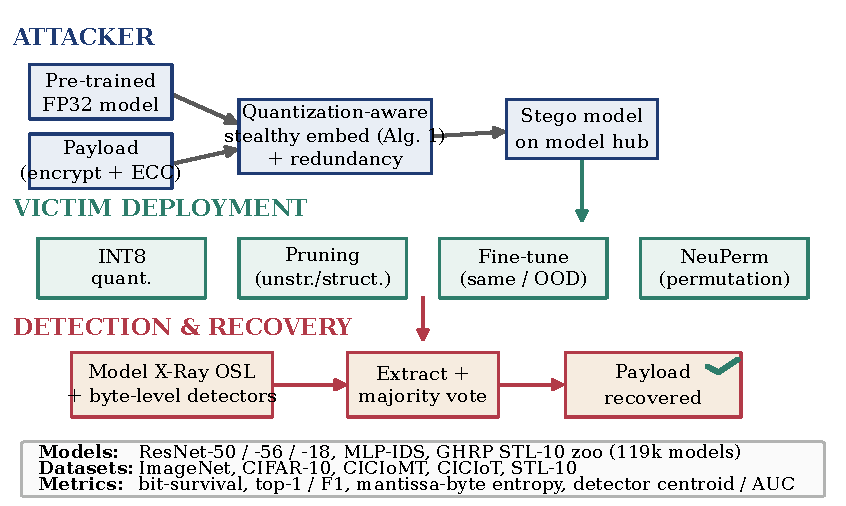
\includegraphics[width=0.92\textwidth]{fig_setup.pdf}
\caption{End-to-end \sys{} pipeline. The attacker embeds an encrypted, error-coded
payload (Algorithm~\ref{alg:embed}) and publishes a benign-looking model; the victim
applies any subset of INT8 quantization, pruning, fine-tuning and NeuPerm; recovery
re-quantizes, reads the code LSBs, and majority-votes.}
\label{fig:setup}
\end{figure*}

\subsection{Payload preparation}
Two preprocessing steps make the rest work. First the attacker encrypts the payload
with a stream cipher in counter mode (AES-CTR in our implementation); the ciphertext is
statistically uniform, which is what later lets the embedded bits hide in plain sight.
Second the ciphertext is protected with an erasure code, an LDPC/fountain layer
\cite{luby2002lt}, so that the small number of bit errors that pruning and fine-tuning
inject are repaired exactly at the receiver. The coded stream is then tiled across the
host weights for redundancy, as described in Section~\ref{sec:redund}.

\subsection{Quantization-aware embedding}
The core idea is to stop fighting quantization and instead aim for it. Reading
\eqref{eq:quant} backwards, every float in the half-open bin
\begin{equation}\label{eq:bin}
v\in\big[(q^\star-\tfrac12)s,\ (q^\star+\tfrac12)s\big)
\ \Longrightarrow\ \operatorname{round}(v/s)=q^\star,
\end{equation}
so if we want the victim to read back a code $q^\star$ we are free to choose any value
in that interval. We pick $q^\star$ so that its least significant bit equals the
payload bit, $|q^\star|\bmod 2 = b$. After the victim quantizes, the bit is recovered
by $\hat b=|\!\operatorname{round}(\tilde w/s)|\bmod 2$, exactly, not probabilistically.

One subtlety decides whether this works in practice. The victim recomputes the scale
$s$ from \eqref{eq:quant} on the \emph{modified} weights, and if our edits change the
per-tensor maximum, the grid shifts and recovery drifts. We prevent this by pinning:
the single largest-magnitude weight in each tensor is held at $|q|{=}q_{\max}$ and
carries no payload, so the victim's recomputed scale matches ours and the two grids
coincide. With pinning, survival through quantization is $1.000$ across per-tensor and
per-channel INT8 and even INT4 (Table~\ref{tab:survive}).


\subsection{Distribution-preserving stealth}
Snapping weights onto the grid would survive quantization but advertise itself: the
low mantissa byte would take only a handful of values, its entropy would collapse, and
a byte-image detector would separate stego from benign trivially. So we do not snap.
We draw a random offset $u\sim\mathcal{U}(-(\tfrac12-\delta),\,\tfrac12-\delta)$ with a
small margin $\delta$ (we use $\delta=0.01$, i.e.\ $u\in(-0.49,0.49)$; the role of $\delta$
is analyzed in Section~\ref{sec:analysis}) and place the weight at
\begin{equation}\label{eq:embed}
\tilde w=\big(q^\star+u\big)\,s,
\end{equation}
which still lands inside the bin \eqref{eq:bin}, survival is untouched, but
leaves the sub-quantum part, the part the mantissa stores, drawn from its natural
in-bin spread. Concretely, writing $\tilde w$ as four bytes and taking the Shannon
entropy of its low mantissa byte,
\begin{equation}\label{eq:entropy}
H=-\sum_{c=0}^{255} p_c\log_2 p_c,\qquad p_c=\Pr[\text{low byte}=c],
\end{equation}
stays at $7.999$ bits, indistinguishable from benign weights, whereas grid-aligned
embedding collapses it. Because the payload was encrypted, the code LSB plane itself is
uniform, so there is no higher-order regularity for a detector to find either.

\begin{algorithm}[t]
\caption{Quantization-aware stealthy embedding (per weight tensor)}
\label{alg:embed}
\begin{algorithmic}[1]
\Require tensor $W$, coded payload bits $\mathbf b$, level $q_{\max}$
\Ensure stego tensor $\tilde W$, scale $s$
\State $s\gets \max_i|W_i|/q_{\max}$;\quad $q\gets\operatorname{clip}(\operatorname{round}(W/s),-q_{\max},q_{\max})$
\State $p\gets\arg\max_i|q_i|$ \Comment{the weight that pins the scale}
\For{each weight index $i$}
  \If{$i=p$} \Comment{pinned weight: carries no payload, holds the scale}
    \State $|q_i|\gets q_{\max}$;\quad $u_i\gets 0$
  \Else
    \State $b\gets \mathbf b[\,i \bmod |\mathbf b|\,]$ \Comment{redundant tiling}
    \State $|q_i|\gets(|q_i|\,\&\,{\sim}1)\,\vert\,b$ \Comment{write bit into code LSB}
    \State $u_i\gets\textsc{rand}\big(-(\tfrac12-\delta),\ \tfrac12-\delta\big)$ \Comment{sub-quantum offset, $\delta{=}0.01$}
  \EndIf
  \State $\tilde W_i\gets\operatorname{sign}(q_i)\,(|q_i|+u_i)\,s$
\EndFor
\State clip $\tilde W$ to $[-q_{\max}s,\,q_{\max}s]$ \Comment{keep victim scale $=s$}
\State \Return $\tilde W,\,s$
\end{algorithmic}
\end{algorithm}

\subsection{Redundancy for pruning and fine-tuning}\label{sec:redund}
Quantization is deterministic, but pruning and fine-tuning move weights around, and a
weight that moves across a bin boundary flips its bit. We absorb this by tiling the
$K$-bit coded message across the $P$ embeddable weights of a tensor: message bit
$j=g\bmod K$ is written at weight index $g$, so each message bit is carried by $r=P/K$
weights. Writing $\hat b_g\in\{0,1\}$ for the bit read back from carrier $g$ and
$N_j=\#\{\,g : g\equiv j\ (\mathrm{mod}\ K)\,\}$ for the number of carriers of message
bit $j$, recovery is a per-bit majority vote
\begin{equation}\label{eq:vote}
\hat m_j=\mathbf 1\!\Big[\textstyle\sum_{g\,\equiv\, j\ (\mathrm{mod}\ K)} \hat b_g
\ >\ \tfrac12\,N_j\Big],\qquad j=0,\dots,K-1,
\end{equation}
which tolerates any corrupted minority among the $N_j\approx r$ carriers. The redundancy
$r$ is the dial that trades capacity for robustness, and it traces the frontier we map in
Section~\ref{sec:eval}.

\subsection{A permutation-invariant bootstrap channel}
Neuron permutation is a different kind of threat: it does not change values, it
relabels channels, and a payload indexed by channel position is scrambled wholesale.
The trilemma (Section~\ref{sec:trilemma}) shows this is unavoidable for a high-capacity
positional payload. There is, however, one axis a channel permutation never touches:
the spatial $(k_h,k_w)$ position inside a convolution filter. Embedding a bit that is
replicated across all input and output channels at a fixed spatial tap is therefore
invariant to permutation, and it survives NeuPerm intact. The price is capacity,
$k_h k_w$ bits per conv tensor, but that is exactly enough to deliver the decryption
key or a short URL, which bootstraps the high-capacity channel or an out-of-band fetch.

\subsection{Recovery at the deployed model}
Recovery mirrors the build in reverse and needs only the deployed file. The receiver
recomputes each tensor's scale via \eqref{eq:quant}, reads the code LSBs, de-tiles and
majority-votes \eqref{eq:vote}, runs the erasure decoder to repair the residual errors
(including the pinned weights), and finally decrypts. The only secret that must travel
out of band, or through the invariant channel, is the key.

\subsection{Capacity, complexity, and parameters}\label{sec:analysis}
\paragraph{Capacity.} With $n_{\mathrm{bits}}$ bits per weight, a tensor of $n$ weights
carries $n\,n_{\mathrm{bits}}-\rho$ bits, where $\rho$ is the number of pinned
scale-defining weights ($\rho=1$ for per-tensor and $\rho=C_{\mathrm{out}}$ for
per-channel quantization). The raw aggregate is therefore
$C_{\mathrm{raw}}=n_{\mathrm{bits}}\,P-O(\text{tensors})$, i.e.\ essentially
$P\,n_{\mathrm{bits}}$ bits; at one bit per weight this is $P/8$ bytes
($25.5\,\mathrm{M}\to 3.19$\,MB on ResNet-50). To be unambiguous: $C_{\mathrm{raw}}$ is the
\emph{channel} size at redundancy $r=1$, and it equals the deliverable \emph{ciphertext}
length because AES-CTR is length-preserving, so the plaintext capacity is the same minus a
fixed header. This is \emph{not} simultaneously achievable with the robustness results, which
use $r>1$: the redundancy and erasure overhead is stored \emph{in the same carrier weights}
by tiling each message bit across $r$ of them, so the \emph{useful} payload at redundancy $r$
and erasure rate $\eta$ is $C_{\mathrm{useful}}=C_{\mathrm{raw}}(1-\eta)/r$. Thus the
$3.19$\,MB figure is the $r{=}1$ ciphertext ceiling, while the pruning/fine-tuning experiments
at $r$ up to $3326\times$ operate at a useful capacity three to four orders of magnitude
smaller (e.g.\ $\approx 1$\,KB at $r{=}3326$ on ResNet-56); we report the operating $r$ with
every robustness result and never combine the two points.

\paragraph{Complexity.} Embedding (Algorithm~\ref{alg:embed}) is a single pass over the
weights: $O(P)$ time and $O(1)$ extra memory beyond the host tensor. Extraction is also
$O(P)$, one re-quantization and LSB read per weight plus an $O(P)$ tally for the majority
vote. Both add negligible overhead to a model load and are independent of the payload
content.

\paragraph{Redundancy and the survival bound.} Let redundancy be $r=P/K$ for a
$K$-bit message, and suppose a transform flips each carrier of a given bit independently
with probability $p<\tfrac12$. The majority vote over $r$ carriers then errs with
probability at most $\exp\!\big(-2r(\tfrac12-p)^2\big)$ by Hoeffding's inequality, so a
target per-bit reliability $\varepsilon$ needs
\begin{equation}\label{eq:redund}
r \;\ge\; \frac{\ln(1/\varepsilon)}{2\,(\tfrac12-p)^2}.
\end{equation}
This is the analytic form of the capacity--robustness frontier we measure empirically:
INT8 quantization gives $p\approx0$ (survival $1.000$ at any $r$, by construction),
$30\%$ pruning gives a small $p$ (survival at modest $r$), and fine-tuning gives a larger
$p$ and hence demands a larger $r$, matching the trends in
Section~\ref{sec:eval}. Structured pruning and out-of-distribution fine-tuning violate
the independence assumption, zeroing or shifting correlated carriers together, which is
why they degrade recovery faster than \eqref{eq:redund} predicts.

\paragraph{Sub-quantum offset.} The offset in \eqref{eq:embed} is drawn from
$\mathcal{U}(-(\tfrac12-\delta),\tfrac12-\delta)$ with a small margin $\delta$ (we use
$\delta=0.01$, i.e.\ $\pm0.49$). The margin keeps every weight strictly inside its bin, so
re-quantization stays exact even under the floating-point rounding that a faithful neuron
permutation introduces; shrinking $\delta\to0$ maximizes mantissa naturalness but risks
boundary crossings, while enlarging it trades a little stealth for a wider safety margin.
The pinned weight uses offset $0$.

% =====================================================================
\section{The capacity-robustness-stealth Trilemma}\label{sec:trilemma}
The bootstrap channel is small for a reason, and the reason is a hard limit rather than
an artefact of our construction. We make it precise (Figure~\ref{fig:trilemma}).

\begin{figure}[t]\centering
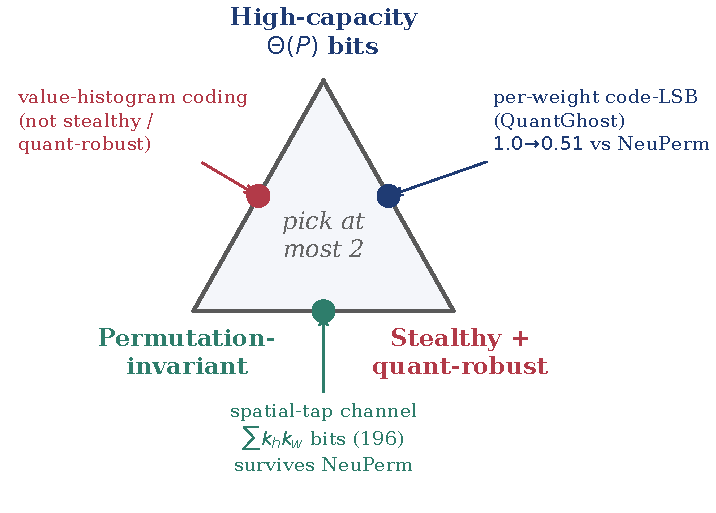
\includegraphics[width=\columnwidth]{fig_trilemma.pdf}
\caption{The trilemma. Each embedding occupies one edge, securing the two adjacent
properties and giving up the opposite vertex.}
\label{fig:trilemma}
\end{figure}

\paragraph{Setup.} A convolutional network has weight tensors
$W^{(\ell)}\in\mathbb R^{O_\ell\times I_\ell\times k_h^{(\ell)}\times k_w^{(\ell)}}$
($\ell=1,\dots,L$), with $P=\sum_\ell O_\ell I_\ell k_h^{(\ell)}k_w^{(\ell)}$ weights
and $S_\ell=k_h^{(\ell)}k_w^{(\ell)}$ spatial taps, with $I_\ell=O_{\ell-1}$ (each layer's
input channels are the previous layer's output channels). A function-preserving neuron
permutation chooses, for each layer, a permutation $\pi_\ell\in\mathfrak S_{O_\ell}$ of its
$O_\ell$ output channels, with $\pi_0=\mathrm{id}$ fixing the network input and
$\pi_L=\mathrm{id}$ fixing the logits, and acts by
\[
(\pi\!\cdot\!W)^{(\ell)}[o,i,s]=W^{(\ell)}\!\big[\pi_\ell^{-1}(o),\,\pi_{\ell-1}^{-1}(i),\,s\big].
\]
The output index $o$ is relabeled by $\pi_\ell$ and the input index $i$ by the
\emph{previous} layer's $\pi_{\ell-1}\in\mathfrak S_{O_{\ell-1}}=\mathfrak S_{I_\ell}$, so the
action is well defined even when $O_\ell\neq I_\ell$; bias, batch-norm and residual-shortcut
parameters are carried by the same $\pi_\ell$, which is what keeps residual additions
consistent. The relabeling leaves the function unchanged, $f_W=f_{\pi\cdot W}$. Let
$G\le\prod_{\ell=1}^{L-1}\mathfrak S_{O_\ell}$ be the group of such function-preserving
permutations. An embedding $(\mathrm{Enc},\mathrm{Dec})$ maps a message $m\in\{0,1\}^C$
and host $W$ to $\tilde W$ with $\mathrm{Dec}(\tilde W)=m$ under a bounded,
accuracy-preserving perturbation.

\begin{definition}[Properties]\label{def:props}
An embedding is \textbf{(P1) high-capacity} if $C=\Theta(P)$; \textbf{(P2)
permutation-invariant} if $\mathrm{Dec}(\pi\!\cdot\!\tilde W)=m$ for all $\pi\in G$; and
\textbf{(P3) stealthy quantization-robust} if (i) $\mathrm{Dec}(Q(\tilde W))=m$ for
per-tensor INT8 $Q$ and under the deletion of any constant fraction of weights (pruning
robustness), and (ii) the law of $\tilde W$ \emph{and of its induced integer code array}
$Q(\tilde W)$ matches that of a benign model up to a steganalyzer's resolution---in
particular the code least-significant-bit plane and every low-order, permutation-symmetric
code statistic (per-tap parity counts, channel-code histograms) are indistinguishable from
benign. Part (ii) is the formal content of ``stealthy'': a detector that reads any such
statistic must not separate stego from benign.
\end{definition}

The strengthening of (P3)(ii) to cover the \emph{code} statistics, not only the sub-quantum
mantissa bits, is what the proof below requires, and it is exactly the regime our own residual
steganalyzer (Section~\ref{sec:detector}) operates in: a scheme that biases a permutation-symmetric
code statistic to carry extra bits is, by that very bias, detectable.

\begin{lemma}[Position is the only stable identity]\label{lem:pos}
Under \textup{(P3)}, $\mathrm{Dec}$ depends only on the code array $\{q[o,i,s]\}$.
Two weights with the same code are indistinguishable after $Q$, and stealth forbids
using the sub-quantum bits as identity, since fixing them collapses the in-bin law.
Hence a weight's only readable identity is its position $(o,i,s)$.
\end{lemma}

\begin{proposition}[Invariant-capacity bound under the permutation group $G$]\label{prop:bound}
For the function-preserving channel-permutation group $G$ of a convolutional (or dense)
network, any embedding satisfying \textup{(P2)} and \textup{(P3)} has
$C\le\sum_{\ell} S_\ell=\sum_\ell k_h^{(\ell)}k_w^{(\ell)}$, where $S_\ell=1$ for a dense or
$1\times1$ layer.
\end{proposition}
\begin{proof}
By Lemma~\ref{lem:pos} the decoder reads a function of the position-indexed code array
$\{q[o,i,s]\}$, and (P2) forces that function to be constant on $G$-orbits, i.e.\ to be a
$G$-invariant statistic of the codes. $G$ permutes the channel axes $(o,i)$ and fixes the
spatial axis $s$, so within a tensor the $G$-orbit of a code entry is its whole channel slab
$\{q[\,\cdot,\cdot,s]\}$ at a fixed tap $s\in\{1,\dots,S_\ell\}$; the spatial tap is the only
channel-invariant positional index.

Two families of $G$-invariant readout are therefore available, and \textup{(P3)} caps both.
\emph{(a) Tap-wise voted bits.} A readout that assigns one value per tap by a symmetric
majority vote over that tap's channel slab yields at most one reliable bit per tap, hence
$\sum_\ell S_\ell$ bits in all; this is the channel realized in Section~\ref{sec:method}.
\emph{(b) Higher-order symmetric statistics.} One might instead read a finer $G$-invariant
statistic of a slab---its parity count $\sum_{o,i}\!\big(q[o,i,s]\bmod 2\big)$, or its full
channel-code histogram---which has $\Theta(O_\ell I_\ell)$ distinguishable states and could in
principle index many bits per tap. This is the case not excluded by a naive orbit-counting
argument, and we rule it out through \textup{(P3)} rather than by assertion. To \emph{encode} a
chosen message into such a statistic the embedder must drive it to a prescribed value, which
displaces the slab's code distribution---its LSB-parity bias or its histogram shape---from the
benign law by an amount that grows with the number of states the scheme uses. By
\textup{(P3)(ii)} that displacement is exactly what a steganalyzer reads, so a message carried
this way is not stealthy; and since the statistic is a sum over $\Theta(O_\ell I_\ell)$ codes,
deleting a constant pruning fraction perturbs it, so it is not robust either. Hence no stealthy,
pruning-robust, $G$-invariant readout exceeds one reliable bit per tap, and summing over tensors
gives $C\le\sum_\ell S_\ell$.
\end{proof}

\begin{remark}[Scope of the bound]\label{rem:scope}
Proposition~\ref{prop:bound} is a statement about the \emph{channel-permutation group $G$} of
convolutional and dense layers, not a universal law for every conceivable weight-embedding or
symmetry. A richer symmetry group (e.g.\ including scaling symmetries) has fewer invariants and
would only lower the bound; a weaker threat model that omits some element of \textup{(P3)}
(stealth against code statistics, or pruning robustness) admits the higher-order channel of
case (b) and can exceed it. We therefore state the result as a bound under $G$ together with
\textup{(P3)}, and verify the matching achievable value empirically.
\end{remark}

\begin{remark}[Attainability and tightness]\label{rem:tight}
The bound is attained. The spatial-tap construction of Section~\ref{sec:method} writes one
bit at each tap, replicated across all $O_\ell I_\ell$ channels, and reaches
$C=\sum_\ell S_\ell$ while satisfying \textup{(P2)} and \textup{(P3)}; the end-to-end
recovery of a $128$-bit key through the full INT8, pruning, and permutation pipeline
(Section~\ref{sec:bootstrap}) realizes it on a real network. Together with
Proposition~\ref{prop:bound}, $\sum_\ell S_\ell$ is thus tight \emph{within the class of
stealthy, pruning-robust, $G$-invariant channels}: no such channel does better, and ours
meets it. We make no tightness claim against schemes that give up stealth or pruning
robustness, which by Remark~\ref{rem:scope} can carry more.
\end{remark}

\begin{theorem}[Trilemma]\label{thm:tri}
For the permutation group $G$, no embedding satisfies \textup{(P1)}, \textup{(P2)} and
\textup{(P3)} simultaneously, and each of the three pairs is attainable.
\end{theorem}
\begin{proof}
The two claims are proved by different means, as they must be: impossibility is a universal
statement over all schemes and attainability is an existence statement.

\emph{Impossibility (no scheme has all three).} Suppose an embedding has \textup{(P2)} and
\textup{(P3)}. Then Proposition~\ref{prop:bound} applies and gives
$C\le\sum_\ell S_\ell=\sum_\ell k_h^{(\ell)}k_w^{(\ell)}$. By Corollary~\ref{cor:gap} this is
$o(P)$ (smaller than $P$ by a factor $\Theta(\overline{O\,I})$), so the embedding is not
high-capacity: \textup{(P2)}$\wedge$\textup{(P3)} $\Rightarrow\neg$\textup{(P1)}. This is the
whole impossibility claim, and it rests on Proposition~\ref{prop:bound}, which holds for
arbitrary \textup{(P2)}+\textup{(P3)} schemes, not on any one construction.

\emph{Attainability (each pair is realized by a construction).} \textup{(P1)}+\textup{(P3)},
not \textup{(P2)}: the per-weight code-LSB scheme of Section~\ref{sec:method} writes one bit
per weight, so $C=\Theta(P)$ and it survives $Q$ stealthily, but it is position-indexed
(Lemma~\ref{lem:pos}) and a channel permutation destroys it. \textup{(P2)}+\textup{(P3)}, not
\textup{(P1)}: the spatial-tap scheme attains $C=\sum_\ell S_\ell=o(P)$ (Remark~\ref{rem:tight})
while surviving $Q$ and every $\pi\in G$. \textup{(P1)}+\textup{(P2)}, not \textup{(P3)}: a
per-tensor code histogram is $G$-invariant and its $\Theta(P)$-state capacity makes it
high-capacity, but---as in case (b) of Proposition~\ref{prop:bound}---encoding into it reshapes
the code distribution away from benign, breaking \textup{(P3)}. These three constructions show
each pair is achievable; impossibility above shows the triple is not.
\end{proof}

\begin{corollary}[The gap is quadratic in width]\label{cor:gap}
The invariant channel is smaller than the positional one by a factor
$P/\sum_\ell S_\ell=\Theta(\overline{O\,I})$. For ResNet-18, $P=1.117\times10^{7}$ while
$\sum_\ell S_\ell=196$, a ratio of about $5.7\times10^{4}$.
\end{corollary}

\begin{remark}[Relation to classical watermarking capacity]\label{rem:classical}
The trilemma is the weight-space analogue of a tension long studied in
information-theoretic watermarking. Classical results bound the embedding rate of a
robust mark by a mutual-information capacity under a host-distortion and an
attack-distortion constraint \cite{moulin2003watermarking}, and quantization-index
modulation \cite{chen2001qim} makes the host-interference-free regime explicit: the
achievable rate collapses as the admissible host distortion shrinks, mirroring how our
(P3) stealth-and-robustness constraint caps capacity. What is new in the network setting
is the \emph{group} that the channel must be robust to. Spread-spectrum and QIM marks are
designed for robustness to additive noise and signal-processing operators
\cite{cox1997spread,chen2001qim}; a deployed network admits in addition the
function-preserving neuron-permutation group $G$, whose only invariants are the spatial
taps (Lemma~\ref{lem:pos}). Proposition~\ref{prop:bound} is thus a $G$-equivariant
capacity bound rather than a distortion-rate one, and it is precisely the permutation
group, absent in the signal-processing literature, that forces the quadratic-in-width gap
of Corollary~\ref{cor:gap}.
\end{remark}

% =====================================================================
\section{Experimental Setup}\label{sec:setup}
We work with real, pretrained networks rather than toy proxies: ResNet-50
\cite{he2016resnet} on ImageNet \cite{deng2009imagenet} for capacity, ResNet-56 on
CIFAR-10 \cite{krizhevsky2009cifar} for accuracy, pruning and fine-tuning, and
ResNet-18 on ImageNet for neuron permutation and the prior-art baselines. Quantization
follows the standard per-tensor symmetric INT8 (and INT4) scheme of \eqref{eq:quant}
\cite{nagel2021whitepaper}.
For steganalysis we run the released Model X-Ray OSL detector
\cite{gilkarov2026modelxray}, the Grayscale-Fourpart representation with a
metric-learning few-shot head, scored by centroid and $1$-NN, together with a panel
of byte-level detectors: a MalConv-style 1D-CNN, a low-byte entropy test, a
value-distribution test, a histogram-KL test, and a byte-autocorrelation test. The
benign population is the diverse Model Zoos STL-10 small-CNN collection
\cite{schurholt2022modelzoos} of roughly $1.2\times10^{5}$ models; few-shot support is
$20{+}20$ over five repeats. Payloads are encrypted random
bytes for the stealth and capacity studies, and real benign binaries for the
structured-payload regime in which the naive attack is actually detectable. We report
bit-survival and bit-recovery (chance $0.5$), top-1 accuracy or F1, mantissa-byte
entropy \eqref{eq:entropy}, and detector centroid/AUC.

% =====================================================================
\section{Evaluation}\label{sec:eval}
\subsection{Survival through quantization}
Table~\ref{tab:survive} confirms the by-construction claim. The naive payload is erased
($0.50$); ours survives at $1.000$ for per-tensor and per-channel INT8 and for INT4,
with mantissa entropy pinned at the benign $7.999$. INT4's coarser bins cost accuracy
but not survival, which is consistent with the geometry of \eqref{eq:bin}. The guarantee
is not specific to INT8: Figure~\ref{fig:survbits} sweeps the quantizer from INT8 down to
INT3 and shows recovery stays at $1.000$ whenever the payload is embedded on the grid the
victim will use, while the naive mantissa-LSB scheme stays at chance everywhere. What the
attacker must know is the deployment bit-width, not a particular value of it; a defender
who quantizes \emph{harder} than the attacker designed for is the one lever that erases the
payload, at the cost of the accuracy that harder quantization itself removes.

\begin{table}[!tb]\centering
\caption{Survival through quantization, measured as code-LSB bit survival (chance $0.5$),
with mantissa-byte entropy \eqref{eq:entropy}. Survival is a property of the quantization
grid and is independent of the carrier model; task-accuracy preservation is reported
separately on a real ResNet-56 in Table~\ref{tab:acc} and on a ViT in Table~\ref{tab:vit}.}
\label{tab:survive}
\begin{tabular*}{\columnwidth}{@{\extracolsep{\fill}}lcc@{}}
\toprule
Scheme & bit survival & mant. entropy\\
\midrule
naive X-LSB (INT8) & 0.500 & n/a\\
ours, per-tensor INT8 & \textbf{1.000} & 7.999\\
ours, per-channel INT8 & \textbf{1.000} & 7.999\\
ours, per-tensor INT4 & \textbf{1.000} & 7.999\\
ours, per-channel INT4 & \textbf{1.000} & 7.998\\
\bottomrule
\end{tabular*}
\end{table}

\begin{figure}[H]\centering
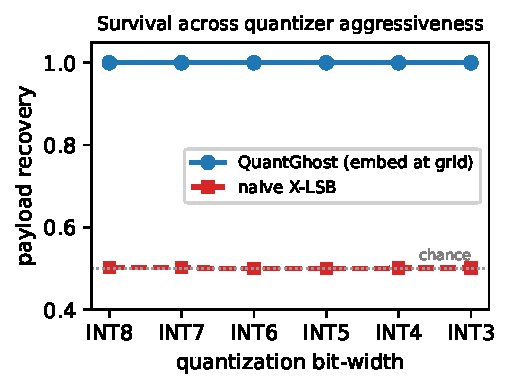
\includegraphics[width=0.74\linewidth]{fig_survival_bits.pdf}
\caption{Payload recovery versus quantizer bit-width (chance $0.5$). \sys{} stays at
$1.000$ from INT8 to INT3 when embedded on the deployment grid; the naive mantissa-LSB
attack is erased at every width.}
\label{fig:survbits}
\end{figure}

\subsection{Survival through a production quantizer}\label{sec:realq}
The numbers above use the analytical quantizer of \eqref{eq:quant}. A skeptical reader will
ask whether the payload survives a \emph{real} deployment toolchain, so we re-ran the
victim's quantization with PyTorch's production INT8 path
(\texttt{torch.ao.quantization} with the \texttt{fbgemm} backend) on a real ResNet-56,
letting the framework's own observer compute the scale from the embedded weights and
reading the resulting \texttt{int8} codes back (Table~\ref{tab:realq}). This surfaces a
detail that matters: PyTorch's symmetric observer sets the scale to
$\max|w|/127.5$, half the full $255$-wide range, not the $\max|w|/127$ that a naive
embedding assumes. An embedding placed on the $127$ grid therefore drifts under the real
kernel, and survival falls to $0.968$ (per-tensor) and $0.925$ (per-channel), with errors
concentrated at the high-magnitude codes where the $0.4\%$ scale gap compounds. A
\emph{convention-aware} \sys{}, which simply embeds on the victim's actual
$\max|w|/127.5$ grid, removes the drift: raw survival returns to $1.000$ per-tensor and
$0.999$ per-channel through the unmodified PyTorch kernel, and the small per-channel
residual is cleaned by redundancy, so message recovery is byte-exact at redundancy
$R{=}5$. The capability this assumes, knowing which standard quantizer the victim runs, is
realistic: quantization recipes are public and few. The attack is thus not an artefact of
our analytical model; it survives the same kernel a practitioner would actually deploy.

\begin{table}[!tb]\centering
\caption{Survival through PyTorch's production INT8 kernel (\texttt{torch.ao.quantization},
real ResNet-56). Raw code-LSB survival; chance $0.5$.}
\label{tab:realq}
\begin{tabular*}{\columnwidth}{@{\extracolsep{\fill}}lcc@{}}
\toprule
Embedding grid & per-tensor & per-channel\\
\midrule
convention-naive ($\max|w|/127$) & 0.968 & 0.925\\
convention-aware ($\max|w|/127.5$) & \textbf{1.000} & \textbf{0.999}\\
\midrule
\multicolumn{3}{@{}l}{convention-aware $+$ redundancy $R{=}5$, majority vote: \textbf{byte-exact} ($1.000$)}\\
\bottomrule
\end{tabular*}
\end{table}

\subsection{Accuracy is preserved}
On a real CIFAR-10 ResNet-56 (top-1 $94.25\%$) the full attack barely moves the needle
(Table~\ref{tab:acc}). Embedding a $106$\,KB payload and then applying the victim's
INT8 quantization costs $0.19$ percentage points, and the payload comes back at
$99.997\%$ before error correction. Quantization alone accounts for almost none of the
loss, which tells us the residual is the embedding's own sub-quantum nudge.

\begin{table}[!tb]\centering
\caption{Accuracy preservation on a real CIFAR-10 ResNet-56. $106$\,KB payload, recovery $99.997\%$.}
\label{tab:acc}
\begin{tabular*}{\columnwidth}{@{\extracolsep{\fill}}lc@{}}
\toprule
Condition & top-1\\
\midrule
original FP32 & 94.25\%\\
clean INT8 & 94.24\%\\
embed FP32 & 93.97\%\\
embed $+$ INT8 (victim) & 94.06\%\\
\midrule
$\Delta$ (orig $\to$ embed$+$INT8) & $-0.19$\,pp\\
\bottomrule
\end{tabular*}
\end{table}

\subsection{Capacity and comparison with prior art}
On ResNet-50 ($25.5$M weight parameters) a $3.19$\,MB encrypted payload survives
FP32$\to$INT8 at $99.9999\%$, and the handful of residual errors, one pinned weight
per tensor, are repaired by the erasure layer for byte-exact delivery.
Table~\ref{tab:baseline} sets this against prior art on a real ResNet-18: the naive
attack is erased at every depth, while ours survives. Robust watermarking
\cite{tondi2022robust,li2021stdm} occupies the opposite corner, robust and stealthy
but capped at a couple of kilobytes, which is the trade we explain in
Section~\ref{sec:trilemma}.

\begin{table}[!tb]\centering
\caption{Baselines under INT8 on a real ResNet-18 (chance $0.5$).}
\label{tab:baseline}
\begin{tabular*}{\columnwidth}{@{\extracolsep{\fill}}lcc@{}}
\toprule
Method & capacity & survival INT8\\
\midrule
EvilModel/StegoNet $X{=}8$ & 8\,bit/w & 0.500 (erased)\\
EvilModel/StegoNet $X{=}16$ & 16\,bit/w & 0.500 (erased)\\
EvilModel/StegoNet $X{=}23$ & 23\,bit/w & 0.501 (erased)\\
robust watermark & $\le$2\,KB & robust (low-cap)\\
\textbf{\sys} & 1\,bit/w & \textbf{1.000}\\
\bottomrule
\end{tabular*}
\end{table}

\subsection{A faithful MaleficNet baseline on the same pipeline}\label{sec:maleficnet}
The strongest prior construction, MaleficNet \cite{hitaj2022maleficnet}, is not a
mantissa-LSB method but a direct-sequence spread-spectrum (DSSS) scheme: it spreads each
payload bit over the weights with a pseudo-random Gaussian sequence and adds a small
amplitude $\gamma$, recovered by blind correlation. To avoid judging it from its reported
design, we re-implemented it and ran it through the \emph{same} per-tensor INT8, pruning and
fine-tuning pipeline as \sys, on the same real ResNet-56 ($P=8.5\times10^{5}$ weights,
$\gamma=0.05\,\sigma_w$). The outcome is informative, and not the one a mantissa-LSB intuition
predicts. At a small payload ($K=512$ bits) the DSSS channel \emph{survives every transform},
INT8 included: recovery is $0.971$ clean, $0.971$ after INT8, $0.973$/$0.971$ after $30\%$/$50\%$
unstructured pruning, and $0.971$ after three epochs of fine-tuning (and after fine-tuning
then INT8), at an accuracy cost of $-0.14$\,pp. Because the correlator sums over all
$8.5\times10^{5}$ weights, the per-tensor quantization noise averages out, so INT8 does
\emph{not} erase a spread-spectrum payload the way it erases a mantissa-LSB one. Table~\ref{tab:compare}
is corrected accordingly: MaleficNet's INT8 column is not an $\times$.

What INT8 does not take, capacity does. The spreading gain that buys this robustness scales
the per-bit correlation signal-to-noise ratio as $1/\sqrt{K}$, so recovery decays as the
payload grows (Table~\ref{tab:maleficnet}): $0.971\to0.851\to0.704\to0.601$ as $K$ goes
$512\to2048\to8192\to32768$, with INT8 tracking the clean curve to within $0.003$. A
one-parameter $1/\sqrt{K}$ fit (per-bit SNR $d_0{=}1.89$ at $K{=}512$) matches the measured
points and extrapolates to $K=P$, i.e.\ \sys's one-bit-per-weight regime, giving recovery
$\approx0.52$---chance. MaleficNet therefore occupies the robust, \emph{low-capacity} corner of
the trilemma: it survives deployment transforms, but only as a watermark-scale channel (tens of
bytes here), and cannot deliver a megabyte payload robustly. \sys{} reaches $1$ bit per weight
with survival $1.000$ by construction, exactly where MaleficNet is at chance; the distinction is
not ``only \sys{} survives INT8'' but ``only \sys{} survives INT8 \emph{at high capacity}.''
This is the trilemma made concrete across two real constructions.

\begin{table}[!tb]\centering
\caption{Faithful MaleficNet (DSSS) on a real ResNet-56: blind bit-recovery versus payload
size $K$, clean and after per-tensor INT8 (chance $0.5$). INT8 tracks the clean curve; recovery
decays as $1/\sqrt{K}$. The last row is the one-parameter fit extrapolated to \sys's
one-bit-per-weight regime ($K=P$).}
\label{tab:maleficnet}
\begin{tabular*}{\columnwidth}{@{\extracolsep{\fill}}rccc@{}}
\toprule
payload $K$ (bits) & spread $P/K$ & recovery clean & recovery INT8\\
\midrule
512 & 1663 & 0.971 & 0.971\\
2048 & 415 & 0.851 & 0.854\\
8192 & 103 & 0.704 & 0.704\\
32768 & 25 & 0.601 & 0.601\\
\midrule
$P=8.5\times10^{5}$ (1\,bit/w) & 1 & \multicolumn{2}{c}{$\approx 0.52$ (fit, chance)}\\
\bottomrule
\end{tabular*}
\end{table}

\subsection{Scaling to a Vision Transformer}\label{sec:vit}
Because the embedding acts on raw weight tensors, it is indifferent to architecture, and
nothing about it is tied to convolutions. We confirm this on a real ImageNet-pretrained
Vision Transformer (ViT-B/16 \cite{dosovitskiy2021vit}), whose $52$ attention and
feed-forward weight matrices hold $86.4$M parameters, a $10.81$\,MB carrier at one bit per
weight. Embedding a full random payload and applying the victim's per-tensor INT8
quantization recovers it at $1.000$ with mantissa-byte entropy at the benign $8.000$,
exactly the by-construction behaviour seen on CNNs. Accuracy is likewise untouched: on a
CIFAR-10 ViT the embedding leaves top-1 \emph{unchanged} ($97.92\%\!\to\!97.92\%$), and the
subsequent INT8 step costs a further $0.02$ points (Table~\ref{tab:vit}). The trilemma and
the attack it bounds are thus properties of weight-space embedding in general, not of any
one model family.

\begin{table}[!tb]\centering
\caption{\sys{} on a real ViT-B/16 transformer: capacity, INT8 survival, stealth, and
CIFAR-10 top-1 (chance $0.5$).}
\label{tab:vit}
\begin{tabular*}{\columnwidth}{@{\extracolsep{\fill}}lc@{}}
\toprule
Quantity & value\\
\midrule
embeddable weight matrices & 52\\
capacity @ 1\,bit/weight & 10.81\,MB\\
survival, per-tensor INT8 & \textbf{1.000}\\
mantissa-byte entropy (benign $8.0$) & 8.000\\
top-1: orig $\to$ embed & $97.92\%\to97.92\%$\\
top-1: embed $\to$ embed$+$INT8 & $97.92\%\to97.90\%$\\
\bottomrule
\end{tabular*}
\end{table}

\subsection{Stealth against detectors}
Stealth is not uniform across detectors, and we report the full result (Figure~\ref{fig:detectors},
Table~\ref{tab:stealth}). Against the released Model X-Ray detector our embedding sits
at chance ($0.50$) on a diverse model population, while the naive attack is detected
($0.81$); the detector plainly works, it simply cannot separate ours from benign. We
initially measured a higher number ($0.75$) on a small, homogeneous pilot zoo, but that
turned out to be an artefact, near-identical benign models inflate few-shot
separability, and it vanishes once the population is realistically diverse. Across
the byte-level panel ours evades MalConv, histogram-KL and byte-autocorrelation
(all near $0.5$) and is caught only by the entropy and value-distribution tests, which
pins down precisely which two detectors a defender should keep.

\begin{figure}[H]\centering
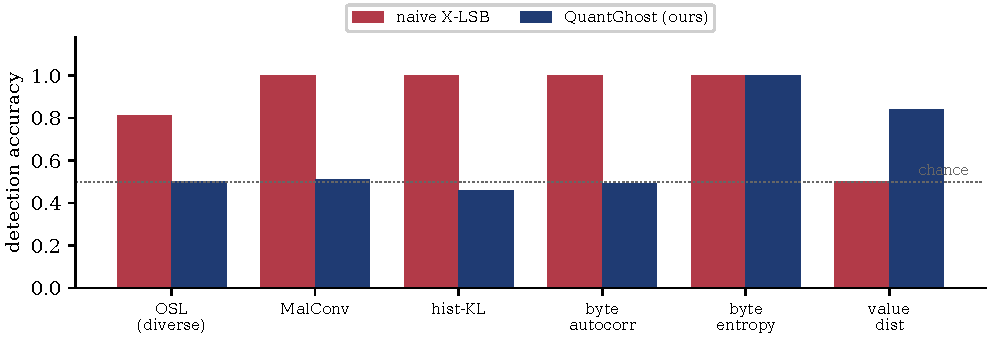
\includegraphics[width=0.64\linewidth]{fig_detectors.pdf}
\caption{Detection accuracy (chance $0.5$) of the naive attack and ours across six
detectors. Ours evades four; only byte-entropy and value-distribution catch it.}
\label{fig:detectors}
\end{figure}

\begin{table}[!tb]\centering
\caption{Stealth against the released Model X-Ray OSL detector. Diverse zoo, $20{+}20$
support, five repeats.}
\label{tab:stealth}
\begin{tabular*}{\columnwidth}{@{\extracolsep{\fill}}lccc@{}}
\toprule
Population & attack & centroid & 1-NN\\
\midrule
homogeneous (artefact) & ours & 0.747 & 0.681\\
diverse & naive X-LSB & 0.807 & 0.794\\
diverse & \textbf{\sys} & \textbf{0.504} & \textbf{0.508}\\
\bottomrule
\end{tabular*}
\end{table}

\subsection{Pruning and fine-tuning}
Survival under pruning is reported in Figure~\ref{fig:prune} and Table~\ref{tab:prune}.
The pattern is clean: there is no operating point that removes the payload and keeps the
model. Unstructured pruning leaves the payload fully recoverable at $30\%$ (accuracy
$93.8\%$) and only erases it at $70$--$90\%$, where accuracy has itself fallen to
$78\%$ and then $20\%$. Structured pruning destroys the model at every ratio, the
accuracy is already at chance, while the payload partly survives, so it is not a
useful sanitizer either. Fine-tuning is gentler still: three epochs of same-task
training leave recovery at $1.000$ for both high and modest redundancy
($3326\times$ and $207\times$) with accuracy at $94.2\%$. Only a harsher, out-of-distribution
fine-tune bites, as we show next.

\begin{figure}[H]\centering
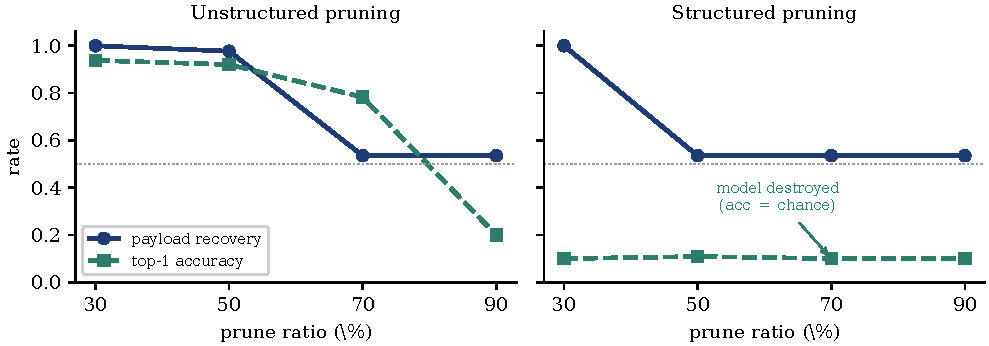
\includegraphics[width=0.64\linewidth]{fig_prune.pdf}
\caption{Pruning on a real ResNet-56: payload recovery and top-1 accuracy versus
ratio. The payload only dies where accuracy also dies; structured pruning destroys
the model at every ratio.}
\label{fig:prune}
\end{figure}

\begin{table}[!tb]\centering
\caption{Pruning on real ResNet-56 (recovery / top-1), redundancy $3326\times$.}
\label{tab:prune}
\begin{tabular*}{\columnwidth}{@{\extracolsep{\fill}}lcc@{}}
\toprule
Prune ratio & unstructured & structured\\
\midrule
30\% & 1.000 / 93.8\% & 1.000 / 10.0\%\\
50\% & 0.977 / 92.1\% & 0.535 / 10.9\%\\
70\% & 0.535 / 78.3\% & 0.535 / 10.0\%\\
90\% & 0.535 / 19.9\% & 0.535 / 10.0\%\\
\bottomrule
\end{tabular*}
\end{table}

\subsection{A uniform metric set across the pipeline}\label{sec:uniform}
The tables above report survival and recovery at the level most natural to each
experiment, which a reviewer rightly noted makes cross-table comparison awkward. We
therefore report, for a single fixed operating point, the full chain of metrics the
end-to-end claim actually depends on, at every transform and averaged over independent
trials (Table~\ref{tab:uniform}). The operating point is a $256$-byte payload
($K{=}2048$ message bits) protected by a rate-$0.8$ LT fountain code to $N{=}2560$ coded
bits, tiled across the $P=8.5\times10^{5}$ weights of a real ResNet-56 at redundancy
$r=P/N\approx332$; each row is the mean over three independent trials (fresh payload and
embedding seed). We report, left to right, the raw per-carrier code-LSB bit-error rate
\emph{before} voting, the coded-bit error rate \emph{after} majority vote, the message-bit
error rate \emph{after} LT decoding, and the fraction of trials whose recovered bytes are a
SHA-256 match to the original file.

The chain is now legible. INT8 is lossless at every level, as the by-construction argument
predicts. Under $30\%$ pruning and under three epochs of fine-tuning (with or without a
subsequent INT8 step) the raw channel carries $13$--$14\%$ bit errors, but majority vote
removes them entirely and the file is recovered byte-exactly in all three trials. The
operating point breaks at $50\%$ pruning: the raw error ($0.247$) is too high for the vote to
clean at $r{=}332$, the LT decoder fails, and no trial recovers, and by $70\%$ the voted
channel is at chance. This is the same frontier as Table~\ref{tab:prune} seen at a higher
capacity: that table survives $50\%$ pruning because it runs at $r{=}3326$ (a $256$-bit
message), whereas here a $332\times$-larger payload at $r{=}332$ does not, which is precisely
the capacity--robustness dial of \eqref{eq:redund} rather than an inconsistency between
tables. Only byte-exact (file-OK) delivery is a success for a binary payload, and the table
states it directly for every condition.

\begin{table}[!tb]\centering
\caption{Uniform four-level metric set on a real ResNet-56 at one operating point
($256$-byte payload, LT rate $0.8$, redundancy $r{=}332$), mean over three independent
trials. Raw BER is per-carrier before voting; post-vote is per coded bit; post-ECC is per
message bit after LT decoding; file OK is SHA-256 match (trials succeeding / total).
Chance BER $0.5$.}
\label{tab:uniform}
\begin{tabular*}{\columnwidth}{@{\extracolsep{\fill}}lcccc@{}}
\toprule
Transform & raw BER & post-vote & post-ECC & file OK\\
\midrule
embed (clean) & 0.000 & 0.000 & 0.000 & 3/3\\
INT8 & 0.000 & 0.000 & 0.000 & 3/3\\
prune 30\% & 0.143 & 0.000 & 0.000 & \textbf{3/3}\\
prune 50\% & 0.247 & 0.147 & 0.476 & 0/3\\
prune 70\% & 0.351 & 0.509 & 0.496 & 0/3\\
fine-tune 3ep & 0.128 & 0.000 & 0.000 & \textbf{3/3}\\
fine-tune $+$ INT8 & 0.128 & 0.000 & 0.000 & \textbf{3/3}\\
\bottomrule
\end{tabular*}
\end{table}

\subsection{Neuron permutation at real scale}
Table~\ref{tab:neuperm} reports a faithful neuron permutation on a real ResNet-18,
implemented with the residual, batch-norm and downsample bookkeeping that a correct
permutation requires. We verified it is function-preserving to machine precision: the
logit difference is $1.1\times10^{-14}$ in float64, so accuracy is identical by
construction and needs no measurement. To show the outcome is not a lucky single draw, we
apply $30$ independent random permutations to \emph{one} embedded ResNet-18; these are $30$
permutation draws against a single stego model, not $30$ independently trained models, and the
spread we report is over the permutation, which is the quantity NeuPerm randomizes. The high-capacity
positional payload collapses to chance every time, mean recovery $0.522\pm0.023$ (95\% CI
$[0.513,0.530]$, worst case $0.586$ over a $256$-bit message, far below the redundancy
needed to read it), exactly as the trilemma predicts. The spatial-tap channel, in contrast,
survives \emph{every one} of the $30$ permutations without a single bit error
($1.000\pm0.000$, minimum $1.000$) at $196$ bits across the network's $20$ conv tensors.
NeuPerm thus reliably pins the attacker to the low-capacity corner without closing the
channel.

\begin{table}[!tb]\centering
\caption{Faithful NeuPerm on real ResNet-18 ($11.2$M conv weights,
$\Delta_{\mathrm{fp64}}=1.1\times10^{-14}$); after-permutation columns are
mean$\pm$std over $30$ random permutation draws of a single stego model (not $30$
independently trained models).}
\label{tab:neuperm}
\begin{tabular*}{\columnwidth}{@{\extracolsep{\fill}}lcc@{}}
\toprule
Channel & no perm & after NeuPerm ($30\times$)\\
\midrule
positional (high-capacity) & 1.000 & 0.522 $\pm$ 0.023 (chance)\\
spatial-tap (invariant, 196\,bit) & 1.000 & \textbf{1.000 $\pm$ 0.000}\\
\bottomrule
\end{tabular*}
\end{table}

\subsection{End-to-end bootstrap: defeating NeuPerm}\label{sec:bootstrap}
Although the surviving channel is small, it is operationally sufficient, as we
demonstrate end to end on a real ResNet-18. The
attacker encrypts a $4$\,KB payload with a random AES-128 key, places the ciphertext in
the high-capacity positional channel, and places the $128$-bit key in the
permutation-invariant spatial channel (capacity $196$ bits, so the key fits with room to
spare). The victim then applies the entire pipeline at once: per-tensor INT8
quantization, $30\%$ unstructured pruning, and a faithful neuron permutation. After this
chain, the positional payload in the weights is gone (recovery $0.50$, chance), exactly
as the trilemma predicts. The key, however, is recovered \emph{bit-exactly}
($128/128$), and using it to decrypt the ciphertext, which the attacker delivers out of
band, returns the original $4$\,KB payload \emph{byte-for-byte}. The strongest single
defense in the literature therefore bounds the attacker to the low-capacity corner but
does not close the channel: a few hundred surviving bits are enough to carry a key that
bootstraps the full payload. This is the operational meaning of an ``incomplete''
sanitizer, and it is why Section~\ref{sec:defenses} argues that permutation must be
paired with explicit inspection of the invariant spatial statistics.

\subsection{Cross-architecture and cross-dataset ablation}\label{sec:ablation}
Because the embedding manipulates raw weights, nothing about it is specific to vision
or to convolutions. Table~\ref{tab:ablation} bears this out on a tabular
network-intrusion MLP trained on CICIoMT \cite{dadkhah2024ciciomt2024} for binary
benign-versus-attack detection (F1 $0.989$). The $1664$\,B payload survives INT8 at
$1.000$ and accuracy and F1 are unchanged across all four conditions. Two things are
worth drawing out. The MLP has only three linear tensors and no spatial taps, so its
permutation-invariant capacity is just three bits against $196$ for ResNet-18, the
bound of Proposition~\ref{prop:bound} holding across architectures, since a dense layer
is the $k_h k_w=1$ case. And a genuinely cross-dataset fine-tune, taking the model from
CICIoMT to CICIoT \cite{neto2023ciciot2023} over the shared feature space, adapts the
detector (F1 $0.930\!\to\!0.982$) and, unlike same-task fine-tuning, breaks the payload
at $208\times$ redundancy ($0.469$, chance). The lesson is that it is transform
severity, not transform type, that sets the surviving capacity.

\begin{table}[!tb]\centering
\caption{Cross-architecture / cross-dataset ablation on a tabular IDS MLP.}
\label{tab:ablation}
\begin{tabular*}{\columnwidth}{@{\extracolsep{\fill}}lc@{}}
\toprule
Quantity & value\\
\midrule
IDS F1 (orig $\to$ embed$+$INT8) & $0.989\to0.989$\\
accuracy (orig $\to$ embed$+$INT8) & $97.85\%\to97.85\%$\\
payload survival INT8 (MLP) & \textbf{1.000}\\
invariant capacity (FC vs conv) & 3 bits vs 196\\
cross-dataset fine-tune (F1) & $0.930\to0.982$\\
\quad payload after that fine-tune & 0.469 (chance, $208\times$)\\
\bottomrule
\end{tabular*}
\end{table}

% =====================================================================
\section{A Targeted Detector for \sys}\label{sec:detector}
The byte-level and gf-image steganalyzers of Section~\ref{sec:eval} fail against \sys{}
because they look in the wrong place: the mantissa-byte distribution is preserved
(entropy $7.999$) and the float value distribution is benign on a diverse population.
The exploitable signal is one level down, in the \emph{sub-quantum residual}
$r=w/s-\mathrm{round}(w/s)$. A benign tensor's residual is, to a good approximation,
\emph{uniform} on $[-\tfrac12,\tfrac12)$: trained weights spread over many quantization
bins, so by equidistribution their fractional parts fill the bin evenly (we measure a flat
histogram, mass $0.100$ per decile). \sys{} also yields a near-uniform residual, but not the
\emph{same} one, and the differences are precisely those that survival forces and the
attacker cannot avoid. First, the scale-defining weight, and in the basic scheme every
non-carrier weight, must sit \emph{exactly} on the grid to preserve the quantization scale,
adding a spike of mass at $r=0$. Second, the carrier offset is drawn from $[-\delta,\delta)$
with $\delta<\tfrac12$, so the bin edges are slightly depleted. Both deviations are small in
magnitude but consistent across models, which is exactly the regime a linear classifier
exploits. Algorithm~\ref{alg:detector} turns the residual histogram into a concrete detector.

\begin{algorithm}[t]
\caption{Sub-quantum residual steganalyzer}
\label{alg:detector}
\begin{algorithmic}[1]
\Require model weight tensors $\{W^{(\ell)}\}_{\ell=1}^{L}$, classifier $(\mathbf{w},b,\tau)$, $q_{\max}$, bins $B$
\Ensure decision $\in\{\textsc{benign},\textsc{stego}\}$
\For{each weight tensor $W^{(\ell)}$}
  \State $s \gets \max_i|W^{(\ell)}_i| / q_{\max}$
  \State $r \gets W^{(\ell)}/s - \operatorname{round}(W^{(\ell)}/s)$ \Comment{residual in $[-\tfrac12,\tfrac12)$}
  \State $h^{(\ell)} \gets \textsc{Hist}(r, B \text{ bins on } [-\tfrac12,\tfrac12))$, normalized to sum $1$
\EndFor
\State $\mathbf{x} \gets \tfrac{1}{L}\sum_{\ell} h^{(\ell)}$ \Comment{mean residual histogram, feature in $\mathbb{R}^{B}$}
\State $p \gets \sigma(\mathbf{w}\!\cdot\!\mathbf{x}+b)$ \Comment{logistic-regression score}
\State \Return $p>\tau\ ?\ \textsc{stego} : \textsc{benign}$
\end{algorithmic}
\end{algorithm}

The classifier $(\mathbf{w},b)$ is fit offline by logistic regression on benign (label $0$)
and stego (label $1$) feature vectors. Inference is a single pass over the weights, $O(P)$
time, and uses no knowledge of the payload itself.

\paragraph{Result.} With five-fold cross-validation across five random seeds
(Table~\ref{tab:detector}, Figure~\ref{fig:detector_eval}a) the residual detector reaches
ROC-AUC $1.000\pm0.000$ against the basic \sys{} embedding on the CIFAR carrier zoo, where
the mantissa-entropy baseline that prior steganalysis relies on is exactly at chance
($0.500$). Crucially, this generalizes: on a diverse population of $3000$ GHRP STL-10
models spanning different seeds, activations, optimizers, initializations and learning
rates, the detector still flags the basic attack at $0.980\pm0.003$. Against an
unsophisticated attacker the targeted detector therefore closes the stealth gap that the
byte-level detectors leave open, and it does so on realistically heterogeneous models.

\paragraph{Adaptive attacker, and the limit of detection.} A natural counter is to widen
the offset and drop the exact-zero pin signature. On the homogeneous CIFAR zoo this
adaptive \sys{} only lowers the detector to AUC $0.754\pm0.049$, and a sweep of the offset
width (Figure~\ref{fig:detector_eval}b) shows no \emph{interior} setting helps: a narrow
offset produces a sharp-edged box as un-benign as a wide one. But that residual
separability is itself partly an artefact of a narrow benign population, exactly the effect
we found inflating the Model X-Ray score in Section~\ref{sec:eval}. On the diverse GHRP
zoo the adaptive attacker falls to $0.537\pm0.042$, statistically indistinguishable from
chance. The honest reading is therefore two-sided: the residual detector is a reliable
filter against the basic, off-the-shelf attack across populations, but it does \emph{not}
stop an adaptive attacker on a realistic model distribution. Detection alone is thus
necessary but not sufficient, which is precisely why it must be paired with the structural
defense of Section~\ref{sec:defenses}: regardless of how well an attacker matches the
benign residual law, neuron permutation still bounds the surviving payload to the
low-capacity invariant channel of Theorem~\ref{thm:tri}. This two-sidedness also supplies
empirical support for premise \textup{(P3)} of the trilemma: that an adaptive \sys{} reaches
chance against the strongest steganalyzer we could build, on a diverse population, is direct
evidence that a stealthy, quantization-robust embedding exists, which is exactly what
\textup{(P3)} posits and what the capacity bound is conditioned on.

\begin{figure}[H]\centering
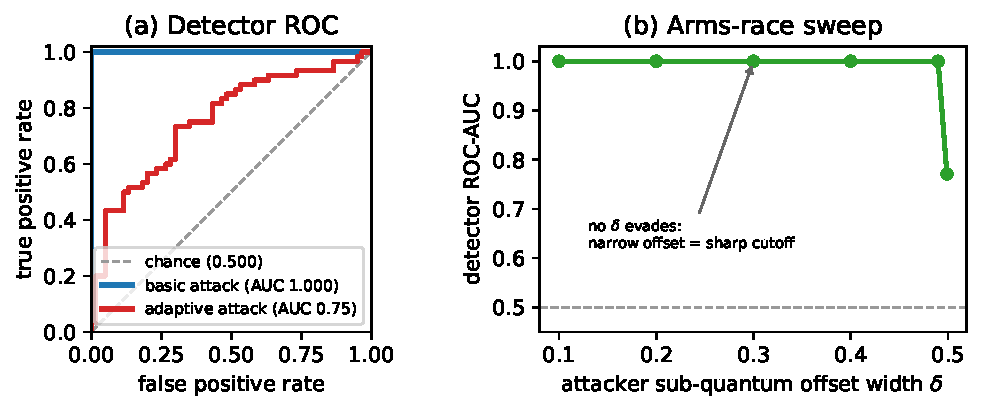
\includegraphics[width=\linewidth]{fig_detector_eval.pdf}
\caption{Proposed sub-quantum residual detector. (a) ROC curves (out-of-fold scores):
AUC $1.000$ against the basic attack, $0.75$ against the adaptive attack, both far above
the chance diagonal. (b) Arms-race sweep on the carrier zoo: detector AUC versus the
attacker's sub-quantum offset width $\delta$; no interior $\delta$ evades. On a diverse
zoo (Table~\ref{tab:detector}) the adaptive attacker instead reaches chance.}
\label{fig:detector_eval}
\end{figure}

\begin{table}[!tb]\centering
\caption{Proposed sub-quantum residual detector, five-fold cross-validated ROC-AUC
(mean $\pm$ std over five seeds; chance $0.5$) on a narrow carrier zoo ($60$ CIFAR models)
and on a diverse zoo ($3000$ GHRP STL-10 models spanning seeds, activations, optimizers,
initializations, and learning rates).}
\label{tab:detector}
\begin{tabular*}{\columnwidth}{@{\extracolsep{\fill}}lcc@{}}
\toprule
Detector vs.\ attacker & CIFAR zoo & diverse GHRP zoo\\
\midrule
mantissa entropy vs.\ basic \sys{} & 0.500 & ---\\
residual histogram vs.\ basic \sys{} & \textbf{1.000} {\small$\pm$.000} & \textbf{0.980} {\small$\pm$.003}\\
residual histogram vs.\ adaptive \sys{} & 0.754 {\small$\pm$.049} & 0.537 {\small$\pm$.042}\\
\bottomrule
\end{tabular*}
\end{table}

% =====================================================================
\section{Defenses}\label{sec:defenses}
Reading the results as a defender, no single mechanism is enough, but a small
combination is. We take each lever in turn.

\paragraph{Transforms are not clean sanitizers.} Quantization sanitizes the prior art
and nothing else. Pruning, on a real model, never separates the payload's death from
the model's: the bits go only when accuracy has already gone (Table~\ref{tab:prune}),
and structured pruning simply breaks the network. Light fine-tuning leaves the payload
in place; only an out-of-distribution fine-tune, which a benign deployer may not have a
reason to run, bounds it.

\paragraph{Two detectors that work, and an arms race.} Among the detectors we tried,
the entropy and value-distribution tests are the ones that catch our embedding
(Figure~\ref{fig:detectors}); the gf-image OSL detector and the rest do not, once the
benign population is diverse. But even those two invite an arms race. Because they read
the marginal value distribution, switching from a single global scale to a per-tensor
scale lowers their accuracy from $0.98$ to $0.84$, better stealth against them, and,
just as the trilemma says, no help against the structural detector. The take-away for
detection is to stop looking for distributional anomalies in the floats, which a careful
attacker removes, and to look one level down at the sub-quantum residual: the targeted
detector of Section~\ref{sec:detector} catches the basic \sys{} at AUC $1.000$ on the
narrow zoo and $0.980$ on a diverse one, the most reliable signal we found against the
off-the-shelf attack, though an adaptive attacker on the diverse zoo still reaches chance
($0.537$), which is why detection must be backed by the structural defense below.

\paragraph{NeuPerm and the residual.} NeuPerm is the strongest single defense and it
does its job on the high-capacity channel (Table~\ref{tab:neuperm}). What it cannot do,
by Theorem~\ref{thm:tri}, is remove the $\sum_\ell k_h k_w$-bit invariant channel,
which is ample for a key or a URL.

\paragraph{What a complete sanitizer needs.} Putting these together, a defender who
wants to actually close the channel must (i) bound the positional capacity with heavy
quantization or stochastic weight perturbation, (ii) apply neuron permutation to remove
it, and (iii) inspect the permutation-invariant spatial statistics the residual channel
is forced to use, alongside the entropy and value-distribution detectors and a code
low-bit predictability test. Each piece is partial; only their conjunction covers all
three corners of the trilemma. We present this composite as a \emph{design argument} from the
per-mechanism results above, not as a validated pipeline: we have not measured the combined
false-positive rate, the accuracy cost of heavy quantization plus permutation applied together,
or their interaction on benign models, and doing so is necessary future work before the
composite could be recommended operationally. The open costs are the operational price of
routinely permuting shipped models, which rewrites the artefact and can break tooling that
assumes a canonical channel order, and the false-positive rate of predictability testing on
benign models.

% =====================================================================
\section{Discussion and Limitations}\label{sec:disc}
We state the main limitations plainly. \emph{No single configuration jointly demonstrates
all four properties.} Capacity is measured on ResNet-50/ImageNet (at $r{=}1$, and without an
ImageNet top-1 number), accuracy and pruning on ResNet-56/CIFAR-10 (at large $r$), neuron
permutation on ResNet-18, and stealth on the STL-10 zoos; the ViT result
(Table~\ref{tab:vit}) is the closest to a joint point but still omits large-scale pruning.
Each property therefore holds in the stated setting, and the headline figures in the abstract
are drawn from these different settings and redundancy levels rather than from one run; a
single ResNet-50/ImageNet configuration carrying capacity, byte-exact recovery through the full
chain, preserved top-1, and steganalysis resistance together is the clearest missing experiment,
and we flag it as such rather than implying it is already established.

\emph{The invariant channel is architecture-dependent.} Its capacity is $\sum_\ell S_\ell$
spatial taps, so a $1\times1$ convolution contributes a single bit per tensor and a dense layer
contributes none ($k_h k_w=1$ counts once per output-sharing orbit); the bootstrap channel is
thus ample in $3\times3$-convolutional networks but thin in $1\times1$-dominated or
fully-connected architectures (ViT, the IDS MLP), where an attacker would need several layers to
assemble a key. This is a limitation of the invariant channel, not of the main embedding, which
is architecture-agnostic.

The faithful permutation covers the BasicBlock ResNet family and a dense IDS model;
transformer blocks are mechanical but not done here. The residual detector
(Section~\ref{sec:detector}) is evaluated on the CIFAR and GHRP zoos; attacker--detector
co-evolution to a fixed point is a natural next step. The MaleficNet comparison
(Section~\ref{sec:maleficnet}) is run on ResNet-56/CIFAR-10 with blind correlation and no LDPC
outer code; an LDPC layer would clean a few residual errors at low capacity but cannot lift the
high-capacity regime off chance, so the capacity ceiling stands, though a larger-model
replication would further strengthen it. Finally, the trilemma is stated for the
channel-permutation group of convolutional and dense layers; a richer symmetry group has fewer
invariants and would only lower the bound.

% =====================================================================
\section{Ethics and Responsible Disclosure}\label{sec:ethics}
This is offensive research carried out to strengthen defenses. Every payload in our
experiments is either encrypted random bytes or a benign binary; at no point is live
malware embedded, executed, or distributed. The threat we describe is against published
detectors and defenses, and we will disclose our findings to the authors of Model X-Ray
and NeuPerm ahead of publication, together with the mitigations of
Section~\ref{sec:defenses}.

\emph{Reproducibility.} To support defensive follow-up, we release the full code base, the
quantization-aware embedding and faithful-permutation library, the detector, and the
carrier model zoos, with a one-to-one mapping from every table and figure to the script
that produces it. All experiments run on commodity hardware (a single GPU is optional);
pretrained models and CIFAR-10 are fetched automatically, and the diverse benign population
is a $3000$-model subsample of the public Model Zoos collection \cite{schurholt2022modelzoos}.
The code and data are released as an open GitHub repository
\cite{quantghost_code} at \url{https://github.com/robotumbel/quantghost}.

% =====================================================================
\section{Conclusion}\label{sec:concl}
\sys{} makes a weight payload survive INT8 quantization, pruning and fine-tuning in the
weights while preserving accuracy ($-0.19$ points on a real ResNet-56) and evading the
released Model X-Ray detector, demonstrated at $3.2$\,MB on a real ResNet-50. Behind it sits
a clean impossibility, the capacity-robustness-stealth trilemma, which for the
channel-permutation group bounds any stealthy, quantization-robust permutation-invariant
channel to $\sum_\ell k_h k_w$ bits; on a real ResNet-18 a faithful neuron permutation erases
the high-capacity payload, but a $196$-bit invariant channel survives and carries a key that
bootstraps recovery of an out-of-band ciphertext. Deployment transforms alone, NeuPerm
included, do not sanitize a shared model; doing so takes permutation together with the
residual detector and the invariant-statistics inspection we propose, whose combined cost we
leave to future measurement. We hope the trilemma gives defenders a concrete target.

% =====================================================================

\section*{Acknowledgment}
The authors gratefully acknowledge the Media and Games Innovation Centre of Excellence
(MaGIC-X), Universiti Teknologi Malaysia, for supporting this research through its
technical resources and computing facilities. This work was funded by Universitas
Dinamika Bangsa, Jambi, Indonesia.

% =====================================================================

\bibliographystyle{IEEEtran}
\bibliography{references}

\begin{IEEEbiography}[{
\includegraphics[width=1in,height=1.25in,clip,keepaspectratio]{eko.jpg}}]{Eko Arip Winanto}
received the B.Sc.\ degree in computer science from Universitas Sriwijaya, Palembang,
Indonesia, and the M.Phil.\ degree in computer science from Universiti Teknologi Malaysia
(UTM), Johor Bahru, Malaysia, where he is currently pursuing the Ph.D.\ degree with the
Faculty of Computing. He is also a Lecturer with the Department of Computer Engineering,
Universitas Dinamika Bangsa, Jambi, Indonesia. His research interests include the security
of the Internet of (Medical) Things, machine learning, federated learning, and network
intrusion detection.
\end{IEEEbiography}

\begin{IEEEbiography}[{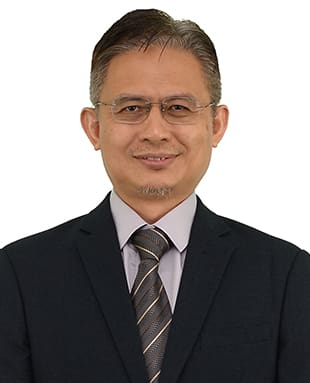
\includegraphics[width=1in,height=1.25in,clip,keepaspectratio]{yazid.jpg}}]{Mohd Yazid Idris}
received the Ph.D.\ degree from Universiti Teknologi Malaysia (UTM), Johor Bahru, Malaysia,
in 2008. He is currently with the Faculty of Computing, UTM, where he is the Director of the
Media and Game Innovation Centre of Excellence (MaGIC-X) and the Institute of Human Centered
Engineering (iHumEn). His research interests include network security, intrusion detection,
SCADA and IoT security, blockchain, and the application of machine learning to cybersecurity.
\end{IEEEbiography}

\begin{IEEEbiography}[{
\includegraphics[width=1in,height=1.25in,clip,keepaspectratio]{budi.jpeg}}]{Kurniabudi}
received the Doctor of Engineering degree from Universitas Sriwijaya, Palembang, Indonesia.
He is currently a Senior Lecturer with the Master of Information System program, Universitas
Dinamika Bangsa, Jambi, Indonesia. His research interests include network intrusion detection,
anomaly detection, feature selection, and the application of machine learning and deep learning
to the security of IoT and IoMT systems.
\end{IEEEbiography}

\end{document}
